\documentclass{article}

% to compile in chinese
\usepackage{CJKutf8}

% if you need to pass options to natbib, use, e.g.:
\PassOptionsToPackage{numbers, compress}{natbib}
% before loading neurips_2024


% ready for submission
% \usepackage{neurips_2024}


% to compile a preprint version, e.g., for submission to arXiv, add add the
% [preprint] option:
%     \usepackage[preprint]{neurips_2024}


% to compile a camera-ready version, add the [final] option, e.g.:
\usepackage[final]{neurips_2024}


% to avoid loading the natbib package, add option nonatbib:
%    \usepackage[nonatbib]{neurips_2024}


\usepackage[utf8]{inputenc} % allow utf-8 input
\usepackage[T1]{fontenc}    % use 8-bit T1 fonts
\usepackage{hyperref}       % hyperlinks
\usepackage{url}            % simple URL typesetting
\usepackage{booktabs}       % professional-quality tables
\usepackage{amsfonts}       % blackboard math symbols
\usepackage{nicefrac}       % compact symbols for 1/2, etc.
\usepackage{microtype}      % microtypography
\usepackage{xcolor}         % colors
\usepackage{graphicx}       % include graphics


\title{具身智能机械臂AI算法实验报告}


% The \author macro works with any number of authors. There are two commands
% used to separate the names and addresses of multiple authors: \And and \AND.
%
% Using \And between authors leaves it to LaTeX to determine where to break the
% lines. Using \AND forces a line break at that point. So, if LaTeX puts 3 of 4
% authors names on the first line, and the last on the second line, try using
% \AND instead of \And before the third author name.


\author{%
  \textbf{学生姓名}: 庄善宁 \\
  \textbf{学号}: 2050828 \\
  \textbf{日期}: 2024.05.28
}

\begin{document}
\begin{CJK*}{UTF8}{gbsn}

\maketitle


\begin{abstract}
本报告设计并实现了一套面向六轴协作机械臂的具身智能AI系统,旨在使其能够理解自然语言指令并自主完成物体的抓取与放置任务。该系统构建了一个模块化的处理流程:首先,利用Kimi大语言模型解析用户指令,提取出操作对象和目标位置;随后,采用OWL-ViT视觉语言模型进行零样本目标检测,从摄像头图像中定位目标物体;接着,通过GraspNet模型结合RGB-D数据预测出稳定可靠的6D抓取位姿;最后,利用ROS中的MoveIt!组件规划并执行无碰撞的机械臂运动轨迹。我们在Mujoco物理仿真环境中对该系统进行了全面验证。在"根据指令将不同颜色的方块放置到对应区域"的任务中,系统在1000次测试中取得了89.6\%的成功率。对失败案例的分析表明,系统的主要挑战在于抓取点不可达、携带物体的路径规划碰撞以及开环控制带来的缺乏动态反馈。本研究完整地展示了如何串联多个前沿AI模型来解决复杂的机器人操作任务,并为未来在真实物理世界中部署和优化此类系统提供了实践性的评估和见解。

\textbf{关键词}: 具身智能;机械臂抓取;大语言模型;视觉语言模型;机器人操作系统(ROS)
\end{abstract}

\section{任务描述}

本次任务的核心目标是为一款六轴协作机械臂搭建一套AI系统,使其能够理解人类的自然语言指令,并自主完成智能化的物体抓取与放置任务。具体而言,该系统需要将用户的口头或书面指令(例如"把红色的方块放到蓝色区域")转化为机器人精确的物理动作。这要求系统具备四大核心能力:

\begin{enumerate}
    \item  \textbf{自然语言理解}:解析用户指令的意图,识别出需要操作的目标物体和目标位置。
    \item  \textbf{视觉感知与目标检测}:通过摄像头识别工作场景,并从中定位到指令中提到的具体物体。
    \item  \textbf{抓取姿态估计}:针对识别出的物体,智能地判断出最合适的抓取位置和姿态,以保证抓取的成功率。
    \item  \textbf{运动规划与执行}:在知晓了抓取目标和最终放置点后,规划出一条从当前位置到目标、再到终点的无碰撞、平滑的运动轨迹,并控制机械臂执行。
\end{enumerate}

整个系统的概念架构如图\ref{fig:concept}所示。
\begin{figure}[h!]
    \centering
    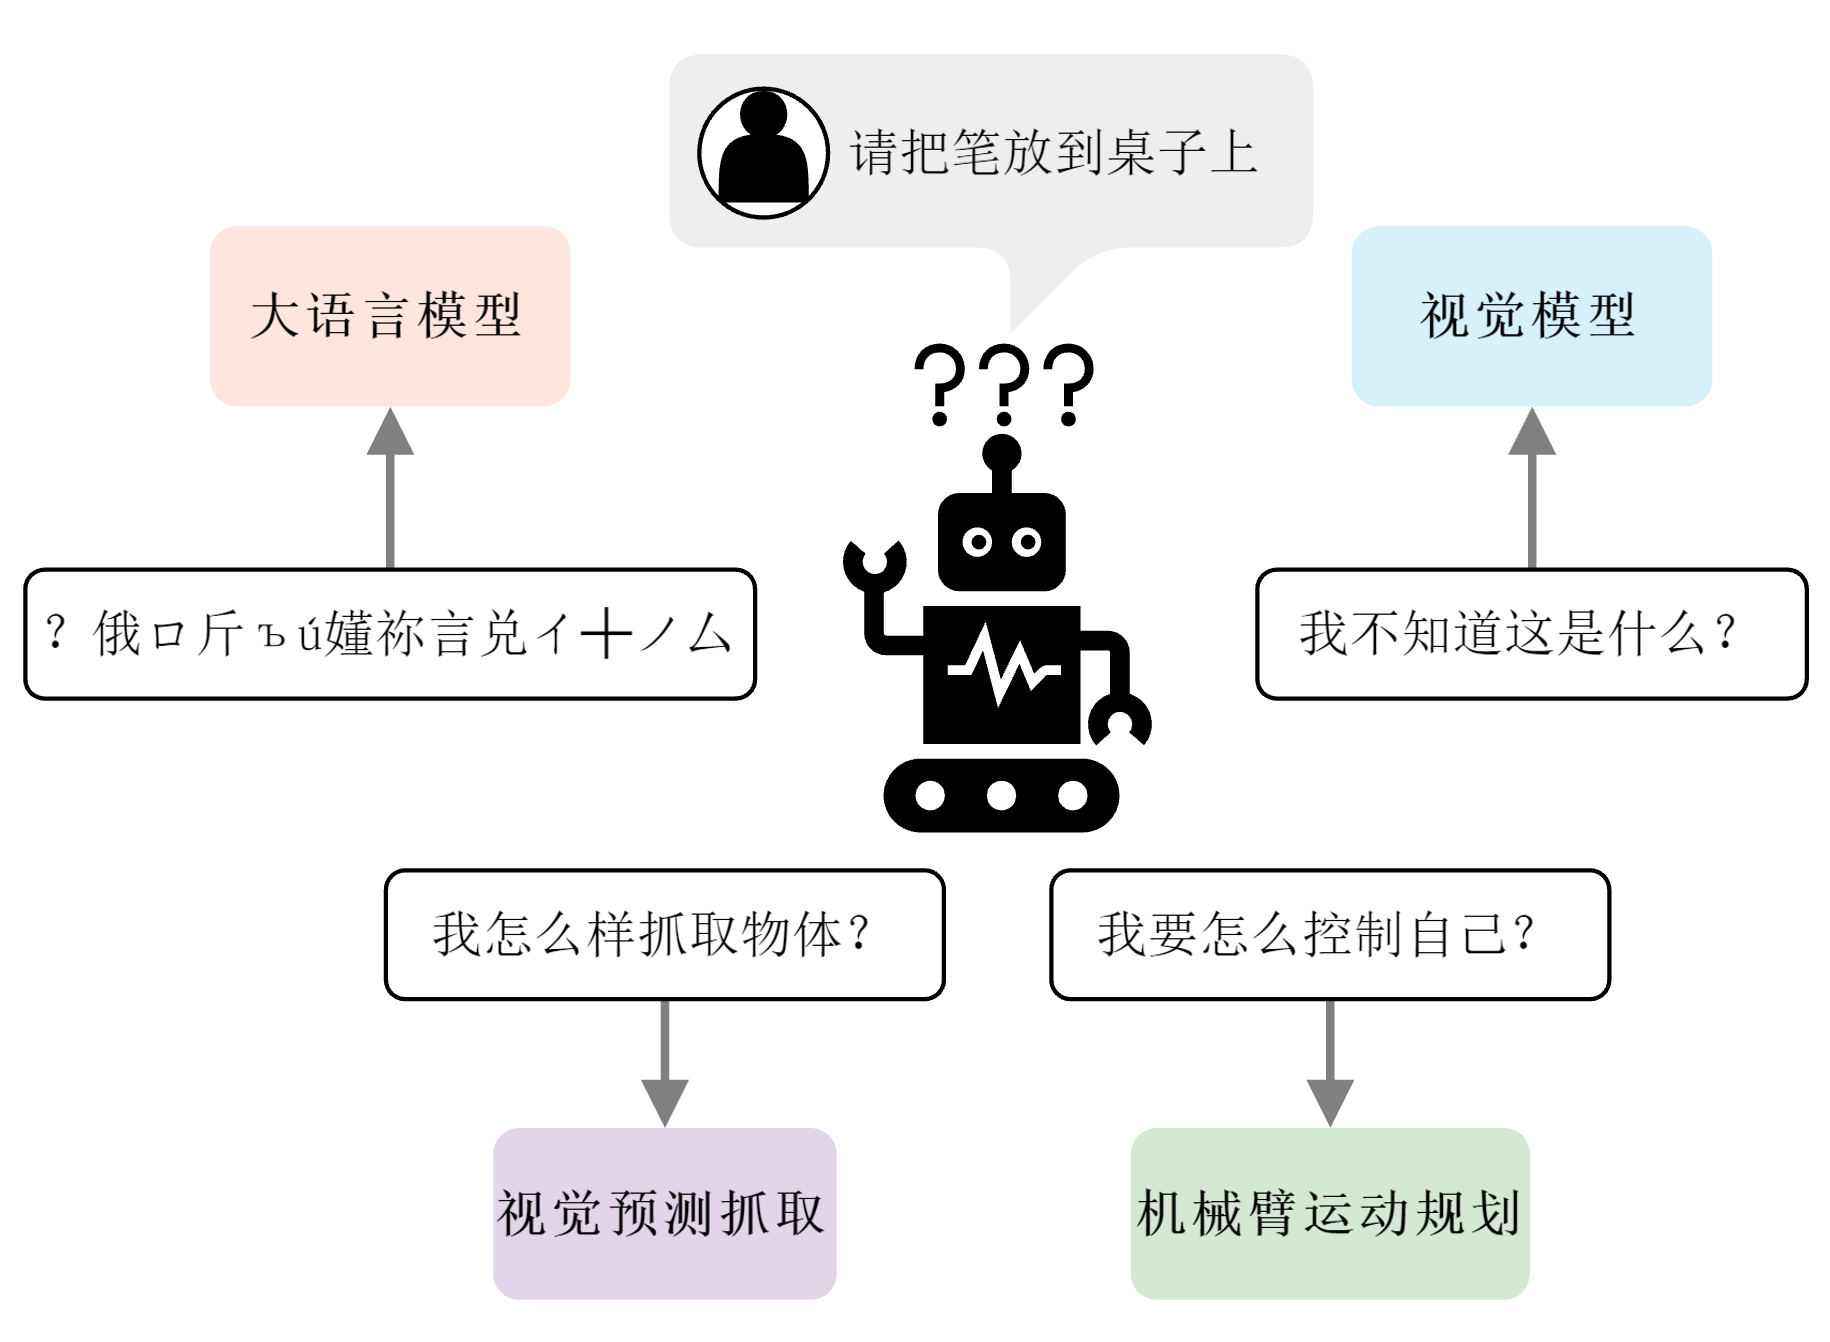
\includegraphics[width=0.8\textwidth]{image/report/1749437532114.png}
    \caption{任务概念图:机械臂根据指令抓取并放置物体。}
    \label{fig:concept}
\end{figure}

\section{具体方法}

为了实现上述任务,我们设计并集成了一个由多个AI模型串联而成的模块化处理流程,整个流程在机器人操作系统(ROS)的框架下进行协调与通信。其算法流程如图\ref{fig:flowchart}所示。

\begin{figure}[h!]
    \centering
    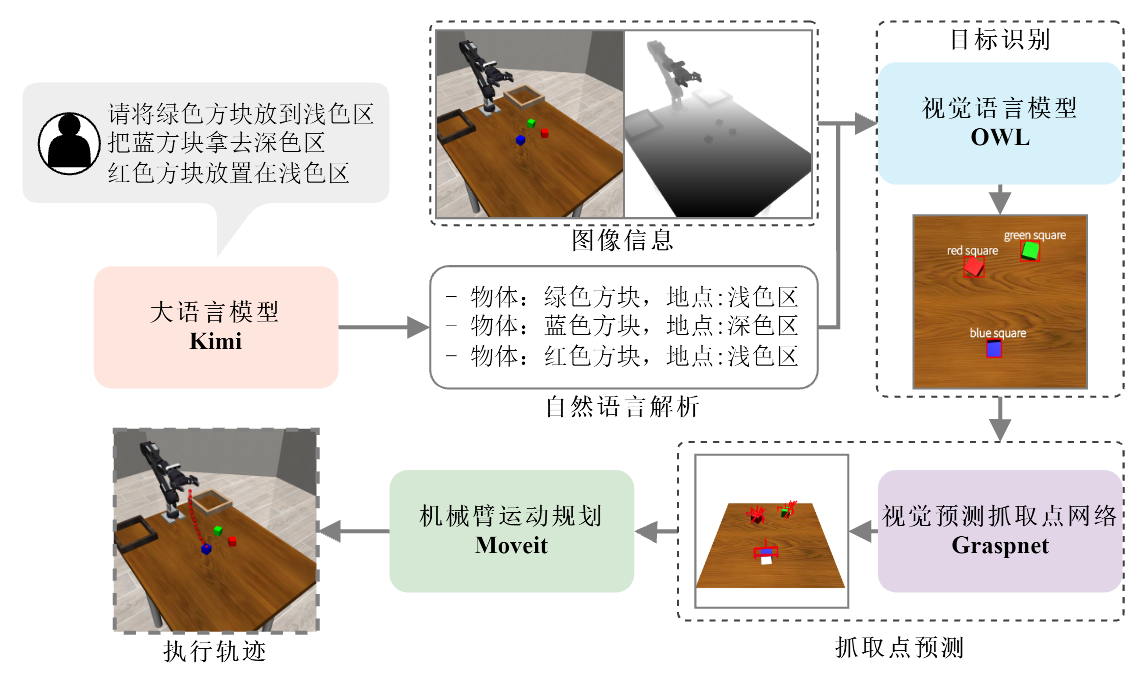
\includegraphics[width=0.8\textwidth]{image/report/1749437542527.png}
    \caption{系统整体算法流程图。}
    \label{fig:flowchart}
\end{figure}

\textbf{各模块详解:}

\begin{enumerate}
    \item  \textbf{指令解析 (大语言模型)}: 用户指令首先被输入到月之暗面公司研发的\textbf{Kimi}大语言模型中。通过精心设计的提示词(Prompt),Kimi能够准确地从自然语言中提取关键信息,并将其格式化为一个JSON对象,例如 \texttt{"{"object": "red block", "destination": "blue area"}"},为后续模块提供结构化的输入(如图\ref{fig:kimi}所示)。
\end{enumerate}

\begin{figure}[h!]
    \centering
    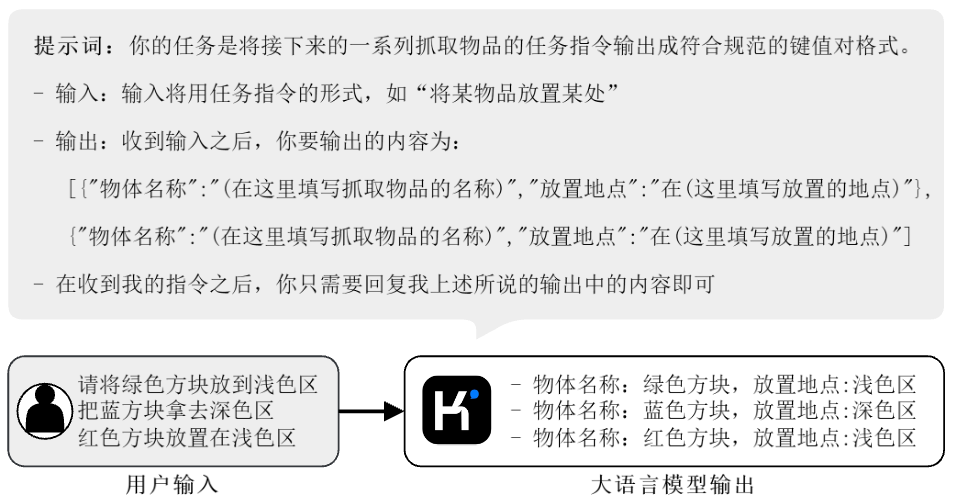
\includegraphics[width=0.8\textwidth]{image/report/1749437549947.png}
    \caption{Kimi大语言模型解析指令,输出结构化JSON。}
    \label{fig:kimi}
\end{figure}

\begin{enumerate}
    \setcounter{enumi}{1}
    \item  \textbf{零样本目标检测 (视觉语言模型)}: 机械臂的摄像头捕捉工作区域的实时图像。随后,Google的\textbf{OWL-ViT (Vision Transformer for Open-World Localization)}模型接收图像和上一步从Kimi解析出的物体名称。OWL-ViT利用其强大的零样本学习能力,即便没有经过特定物体的训练,也能在图像中准确地定位出目标物体,并输出其2D边界框坐标(如图\ref{fig:owlvit}所示)。
\end{enumerate}

\begin{figure}[h!]
    \centering
    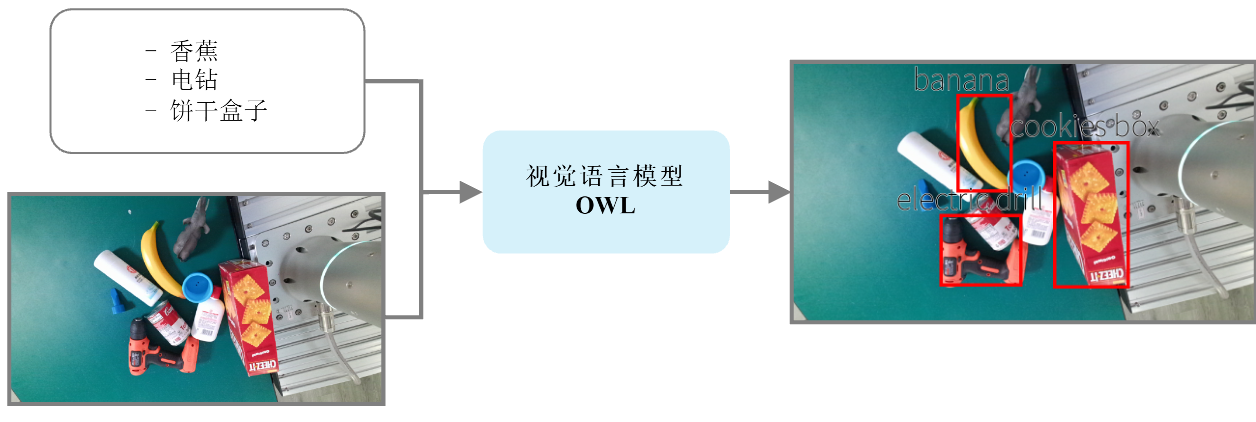
\includegraphics[width=0.8\textwidth]{image/report/1749437557095.png}
    \caption{OWL-ViT根据文本描述进行零样本目标检测。}
    \label{fig:owlvit}
\end{figure}

\begin{enumerate}
    \setcounter{enumi}{2}
    \item  \textbf{抓取姿态预测 (GraspNet)}: 在获得物体的2D位置后,\textbf{GraspNet}模型登场。它结合了RGB图像和深度图像(RGB-D),对目标物体的三维几何形状进行分析,并从中预测出多个可能的、稳定的6D抓取位姿(包括三维空间坐标和三维抓取姿态)。系统会从中选择一个最优的抓取点(如图\ref{fig:graspnet}所示)。
\end{enumerate}

\begin{figure}[h!]
    \centering
    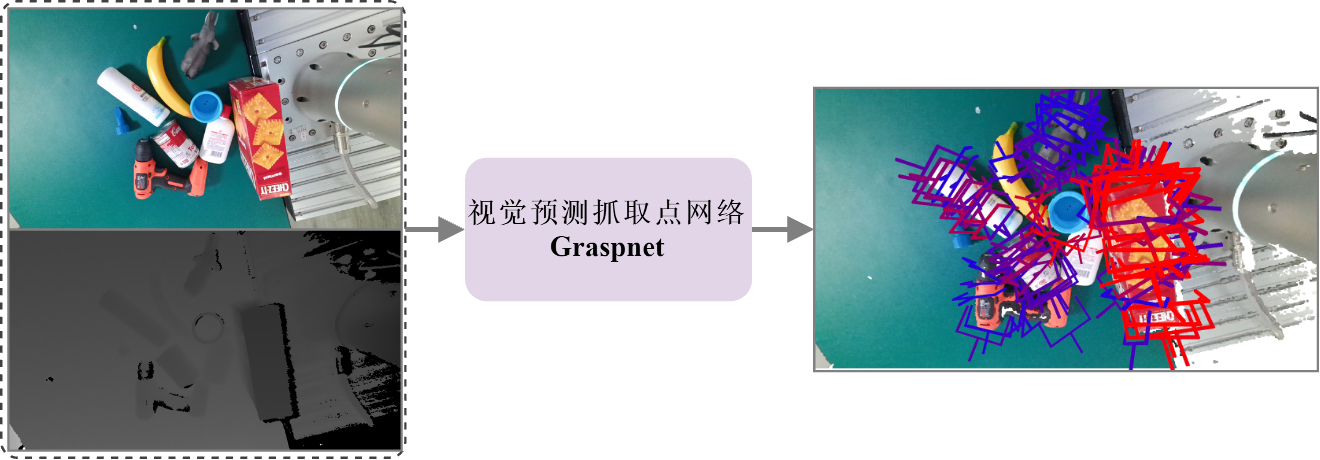
\includegraphics[width=0.8\textwidth]{image/report/1749437564396.png}
    \caption{GraspNet结合RGB-D图像预测6D抓取位姿。}
    \label{fig:graspnet}
\end{figure}

\begin{enumerate}
    \setcounter{enumi}{3}
    \item  \textbf{轨迹规划 (MoveIt)}: 预测出的抓取位姿是基于相机坐标系的,需要先将其转换到机械臂的基坐标系下。然后,这个目标位姿被传递给ROS中的核心运动规划组件\textbf{MoveIt}。MoveIt结合了机械臂的URDF(统一机器人描述格式)模型,综合考虑了运动学、动力学和环境中的障碍物信息,计算出一条平滑且无碰撞的运动轨迹,最后将轨迹点序列通过CAN总线发送给机械臂的各个关节电机,驱动机械臂完成最终的抓取和放置动作(如图\ref{fig:moveit}所示)。
\end{enumerate}

\begin{figure}[h!]
    \centering
    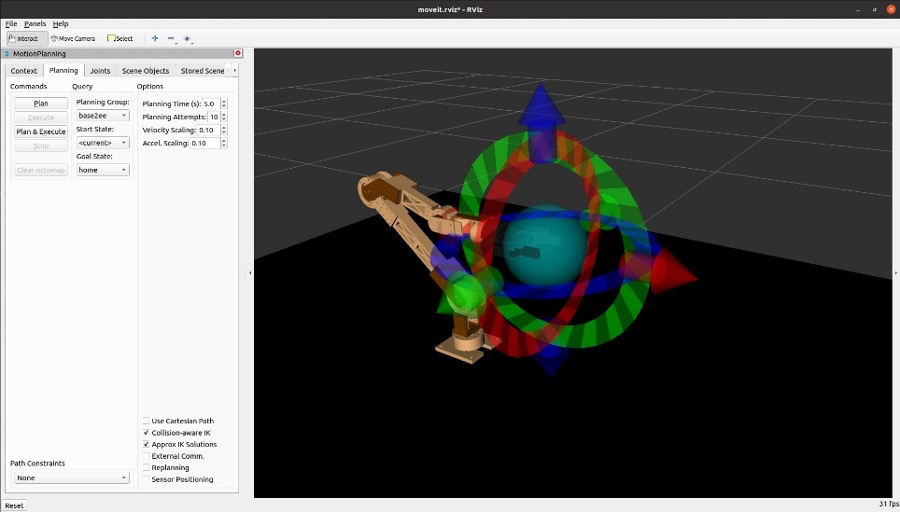
\includegraphics[width=0.8\textwidth]{image/report/1749437570789.png}
    \caption{MoveIt!进行运动规划,生成无碰撞轨迹。}
    \label{fig:moveit}
\end{figure}

\section{结果描述}

我们在\textbf{Mujoco}物理仿真环境中对整套AI算法流程进行了验证。实验任务设定为:将桌面上随机摆放的红、绿、蓝三种颜色的方块,根据指令放置到对应的区域(实验场景如图\ref{fig:sim}所示)。

在总计\textbf{1000次}的仿真实验中,系统成功完成抓取和放置任务的成功率为\textbf{89.6\%}。

对失败案例的分析表明,问题主要源于以下几个方面:
\begin{itemize}
    \item   \textbf{抓取点不可达}:GraspNet预测出的抓取位姿虽然理论上稳定,但有时超出了机械臂的实际工作范围或处于奇异点附近,导致运动规划失败。
    \item   \textbf{路径碰撞}:当方块堆叠或距离过近时,MoveIt在规划路径时,虽然能避免机械臂本体与障碍物碰撞,但有时会忽略夹爪上"携带"的方块的体积,导致在移动过程中,被抓取的方块碰到了桌面上的其他方块,造成任务失败。
    \item   \textbf{缺乏闭环反馈}:系统采用"开环"执行模式,即在任务开始时拍摄一张照片进行决策,执行过程中不再接收视觉反馈。这导致如果中途发生意外(如上文提到的碰撞),系统无法进行动态调整,从而导致连锁失败。
\end{itemize}

\begin{figure}[h!]
    \centering
    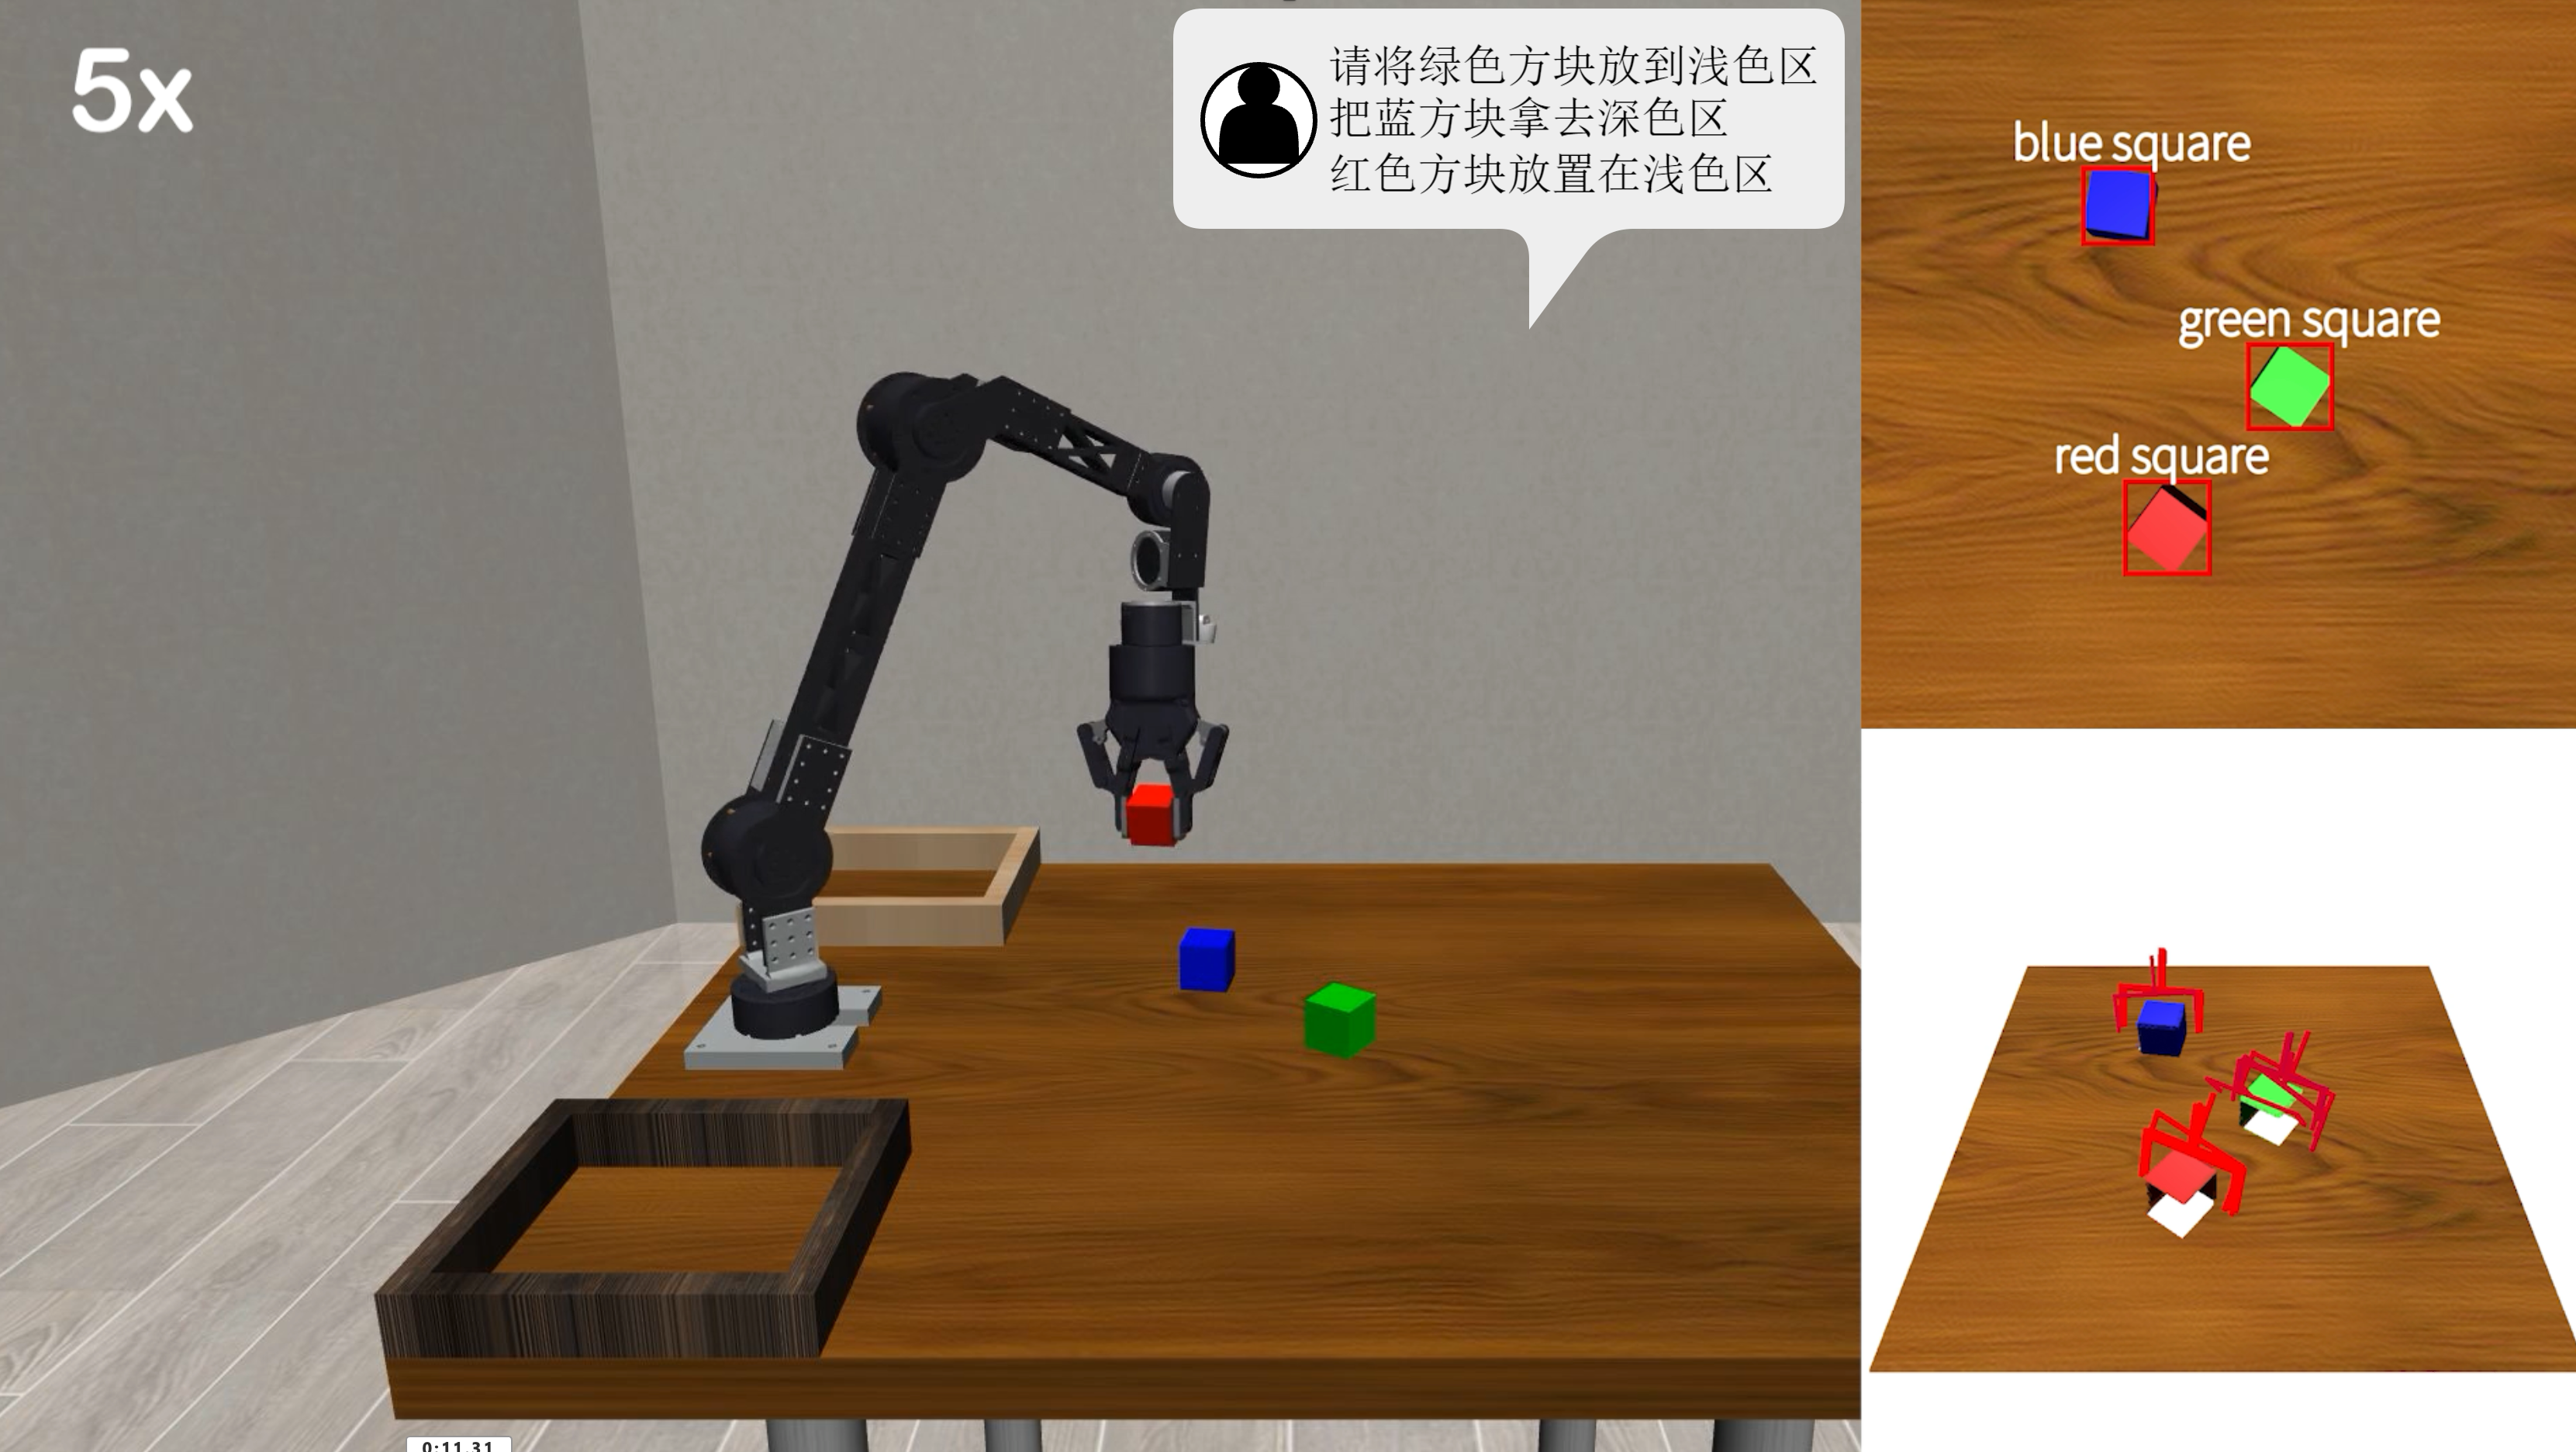
\includegraphics[width=0.8\textwidth]{image/report/1749437618596.png}
    \caption{Mujoco仿真环境中的抓取任务场景。}
    \label{fig:sim}
\end{figure}

\section{体会与建议}

\subsection{对本次任务的体会}

本次大作业是一次将前沿AI技术与机器人学深度结合的宝贵实践。最大的体会是,现代AI的发展,尤其是大模型的出现,正在颠覆传统的机器人编程范式。过去需要为每个任务编写复杂、僵硬的控制代码,而现在我们可以通过组合不同的预训练模型,构建一个能"理解"和"感知"的智能系统,极大地提高了开发的效率和机器人的智能化水平。

然而,实践过程也让我深刻认识到,将多个AI模型"粘合"成一个可靠的系统远非易事。挑战不仅在于单个模型的性能,更在于模型之间的"接口"和"协作"。例如,如何处理坐标系转换的精度问题,如何保证上一个模型的输出是下一个模型的有效输入,以及如何设计一套容错机制来应对某个模型的偶然失效,这些都是工程实践中必须解决的关键问题。

总的来说,这个任务让我从一个更高的维度理解了具身智能——它不仅是算法,更是一个需要软硬件协同、算法与物理世界交互的复杂系统工程。

\subsection{对课程的后续建议}

结合本次毕业设计的经验,我对后续课程提出以下几点建议:

\begin{enumerate}
    \item  \textbf{开设《机器人系统集成》课程}:目前多数课程都专注于单个领域,如"机器学习"或"控制理论"。但如何将这些知识融会贯通,构建一个完整的机器人应用,是学生们普遍欠缺的能力。建议开设一门以项目为导向的系统集成课程,重点讲授\textbf{ROS}等框架的使用,以及多传感器数据融合、多模块通信和软硬件接口调试等实践技能。
    \item  \textbf{加强"仿真到现实 (Sim-to-Real)"的教学}:本次任务的AI算法在仿真中取得了不错的成果,但要将其部署到真实机械臂上,必然会遇到模型不准、延迟、噪声等新问题。建议在课程中加入"Sim-to-Real"相关内容,介绍领域自适应、系统辨识、鲁棒控制等技术,帮助学生填平仿真与现实之间的鸿沟。
    \item  \textbf{鼓励跨学科合作}:具身智能是一个典型的交叉学科领域。可以设计一些需要计算机、机械、电子等不同专业背景学生共同完成的课程项目,让他们在合作中学习如何从系统角度思考问题,并了解不同学科的思维方式和工作流程。这对于培养能够应对未来复杂工程挑战的综合性人才至关重要。 
\end{enumerate}

\end{CJK*}
\end{document}